\chapter{Composants de base} \label{chap:basic_components}
D\'etail des composants de base et leur comportement. Cette section s'inspire du cours d'\'el\'ectrocin\'etique donn\'e par Jimmy Roussel \`a l'ENSCR \autocite{femto-phy}.

\section{Condensateurs} \label{sec:capacitors}
Un condensateur stocke de l'\'energie dans un champ \'electrique entre deux armatures s\'epar\'ees par un isolant (le di\'electrique). Sa relation fondamentale est~:
\[
Q = C \cdot U
\]
où \(C\) est la capacit\'e en farads (\unit{\farad}).
Les condensateurs laissent passer les signaux variables (AC) et bloquent les signaux constants (DC). Ils sont utilis\'es pour filtrer les alimentations, r\'ealiser des circuits r\'esonants, ou encore d\'ecoupler des \'etages \'electroniques. Les types de condensateurs courants incluent~:
\begin{itemize}
  \item \textbf{Condensateurs c\'eramiques~:} petit format, faible ESR (r\'esistance \'equivalente en s\'erie), haute fr\'equence.
        Utilis\'es pour d\'ecouplage, filtrage HF et circuits r\'esonants.
  \item \textbf{Condensateurs \'electrolytiques~:} grande capacit\'e, polarit\'e à respecter,
        adapt\'es au filtrage d'alimentation et au stockage d'\'energie.
  \item \textbf{Condensateurs à film~:} faible perte, non polaris\'es, haute stabilit\'e.
        Applications~: circuits audio, filtres, temporisations.
  \item \textbf{Condensateurs tantale~:} compacts et stables, polarit\'e à respecter,
        utilis\'es pour alimentation stable et d\'ecouplage.
  \item \textbf{Supercondensateurs / ultracapacitors~:} tr\`es grande capacit\'e, d\'echarge rapide,
        pour sauvegarde d'\'energie ou alimentation tampon.
  \item \textbf{Condensateurs à mica~:} grande pr\'ecision, faible perte, haute fr\'equence.
        Utilis\'es pour oscillateurs HF et circuits radio.
  \item \textbf{Condensateurs variables~:} capacit\'e r\'eglable m\'ecaniquement ou \'electroniquement,
        pour syntonisation\footnote{Glossaire~: \gls{syntonisation}}  d'oscillateurs ou ajustement de filtres.
\end{itemize}
\begin{Note}
	Les notions de filtrage, fr\'equences et imp\'edances seront abord\'ees dans la section (Work In Progress) \Cref{subsec:ac_circuit_theory}.
\end{Note}
\textbf{Association en s\'erie~:}
\begin{figure}[H]
    \centering
    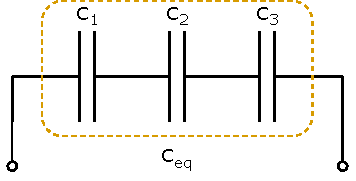
\includegraphics[width=0.6\textwidth]{capacitor-series.pdf}
    \caption{\centering
    Association en s\'erie de condensateurs.\\
    L'inverse de la capacit\'e \'equivalente est la somme des inverses des capacit\'es individuelles
    ~:\\
    \vspace{\baselineskip}
    \(\dfrac{1}{C_{eq}} = \dfrac{1}{C_1} + \dfrac{1}{C_2}\)}
\end{figure}
\textbf{Association en parall\`ele~:}
\begin{figure}[H]
    \fcapside[\FBwidth]{%
        \caption[Condensateurs en parall\`ele.]{
        Association en parall\`ele de condensateurs.\\
        La capacit\'e \'equivalente est la somme des capacit\'es individuelles~:\\
        \(C_{eq} = C_1 + C_2\).}%
        \label{fig:capacitor-parallel}%
    }{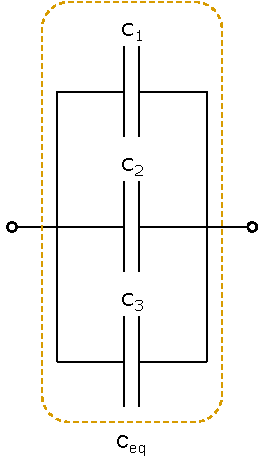
\includegraphics[width=0.4\textwidth]{capacitor-parallel.pdf}}%
\end{figure}

\section{Inductances} \label{sec:inductors}
Une inductance (ou bobine) est un composant passif qui stocke de l'\'energie dans un champ magn\'etique lorsqu'un courant la traverse.
\[
u(t) = L \frac{di(t)}{dt}
\]
où \(L\) est l'inductance (en henrys, \unit{\henry}) et \(i(t)\) le courant instantan\'e.
\vspace{\baselineskip}
Lorsque le courant est constant (\(\frac{di}{dt} = 0\)), la tension aux bornes de l'inductance est nulle (\(u = 0\)). Autrement dit, une inductance se comporte comme un \textbf{court-circuit id\'eal} en r\'egime continu. L'inductance ne s'oppose donc pas au courant constant, mais uniquement aux variations de courant et \'emet un champ magn\'etique constant.

\section{Diodes} \label{sec:diodes}
Une diode est un composant semi-conducteur qui laisse passer le courant dans un sens (polarisation directe) et le bloque dans l'autre (polarisation inverse). Sa caract\'eristique \(I(V)\) est non lin\'eaire et se rapproche d'un interrupteur dirig\'e.
\begin{figure}[H]
    \centering
    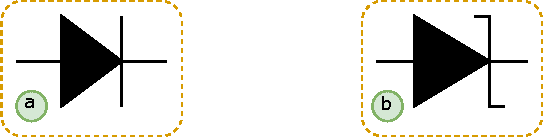
\includegraphics[width=0.5\textwidth]{diodes.pdf}
    \caption{\newline
        \fakecustommacro{a} Symbole d'une diode.\\
        \fakecustommacro{b} Symbole d'une diode Zener.
    }
\end{figure}
Les applications courantes impliquent le redressement dans les alimentations, la protection contre l'inversion de polarit\'e ou la r\'egulation de tension (diodes Zener). Certaines diodes sp\'eciales, comme les LED, convertissent l'\'energie \'electrique en lumi\`ere.

\section{Transistors} \label{sec:transistors}
Le transistor est un composant actif central de l'\'electronique moderne. Il peut amplifier un signal ou agir comme un interrupteur contrôl\'e. On distingue principalement~:
\begin{itemize}
  \item \textbf{BJT (bipolaire)}~: le courant de base contrôle le courant de collecteur.
  \item \textbf{MOSFET (à effet de champ)}~: la tension de grille contrôle le courant de drain.
\end{itemize}
\begin{figure}[H]
    \centering
    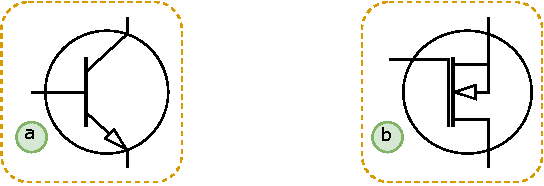
\includegraphics[width=0.6\textwidth]{transistors.pdf}
    \caption{\centering\newline
        \fakecustommacro{a} Symbole d'un transistor NPN (BJT).\\
        \fakecustommacro{b} Symbole d'un transistor N-channel (MOSFET).
    }
\end{figure}
Les transistors sont utilis\'es dans les amplificateurs, les circuits logiques, les r\'egulateurs, et constituent les briques de base des processeurs.
